% =====================================================================
% Project: Software Engineering (DLMCSPSE01)
% Portfolio Part 2 -- Development / Reflection Phase
% Revised full document: Phase 1 content updated after tutor feedback,
% plus the artifacts additionally required in Phase 2.
% Compile: pdflatex <file>.tex  (run TWICE for contents and references)
% Requires: logo.png in the same directory
% =====================================================================
\documentclass[a4paper,11pt]{article}

\usepackage[top=2cm, bottom=2cm, left=2cm, right=2cm]{geometry}
\usepackage[utf8]{inputenc}
\usepackage[T1]{fontenc}
\usepackage{helvet}
\renewcommand{\familydefault}{\sfdefault}
\usepackage{setspace}
\onehalfspacing
\usepackage{parskip}
\setlength{\parskip}{6pt}
\setlength{\parindent}{0pt}
\usepackage{graphicx}
\usepackage{tikz}
\usetikzlibrary{shapes.geometric, arrows.meta, positioning, calc, fit, backgrounds}
\usepackage{booktabs}
\usepackage{tabularx}
\usepackage{longtable}
\usepackage{hyperref}
\hypersetup{colorlinks=true, linkcolor=black, citecolor=blue, urlcolor=blue}
\usepackage[round]{natbib}
\usepackage{fancyhdr}
\usepackage{caption}
\usepackage{subcaption}
\captionsetup[subfigure]{list=false}
\usepackage{enumitem}
\usepackage{xcolor}
% colortbl, NOT xcolor's [table] option -- TikZ already loads xcolor.
\usepackage{colortbl}
\usepackage{float}
\usepackage{array}
\usepackage{amsmath}
\usepackage{xurl}

\pagestyle{fancy}
\fancyhf{}
\fancyfoot[C]{\thepage}
\renewcommand{\headrulewidth}{0pt}

\usepackage{titlesec}
\titleformat{\section}{\normalfont\fontsize{12}{14}\bfseries}{\thesection}{1em}{}
\titleformat{\subsection}{\normalfont\fontsize{11}{13}\bfseries}{\thesubsection}{1em}{}
\titlespacing*{\section}{0pt}{10pt}{4pt}
\titlespacing*{\subsection}{0pt}{8pt}{3pt}

% ---------- Diagram styles ----------
\tikzset{
  system/.style = {draw, rounded corners=2pt, align=center, fill=blue!12,
                   draw=blue!55, minimum width=3.6cm, minimum height=1.2cm,
                   font=\scriptsize\bfseries, inner sep=4pt},
  actor/.style  = {draw, ellipse, fill=gray!12, align=center,
                   font=\scriptsize, inner sep=3pt},
  ext/.style    = {draw, rounded corners=2pt, align=center, fill=gray!12,
                   font=\scriptsize, minimum height=0.8cm, inner sep=4pt},
  flow/.style   = {-{Latex[length=2mm]}, thick, draw=black!65},
  dep/.style    = {-{Straight Barb[length=2.4mm]}, dashed, draw=black!70},
  card/.style   = {draw=black!35, fill=white, rounded corners=2pt,
                   align=center, font=\tiny, minimum width=2.9cm,
                   minimum height=0.62cm, inner sep=2pt}
}

% UML component icon; the coordinate given is the icon's right edge.
\newcommand{\compicon}[2]{%
  \begin{scope}[shift={(#1,#2)}, draw=black!55, line width=0.4pt]
    \fill[white] (-0.24,-0.09) rectangle (0,0.09);
    \draw        (-0.24,-0.09) rectangle (0,0.09);
    \fill[white] (-0.30,0.015) rectangle (-0.18,0.065);
    \draw        (-0.30,0.015) rectangle (-0.18,0.065);
    \fill[white] (-0.30,-0.065) rectangle (-0.18,-0.015);
    \draw        (-0.30,-0.065) rectangle (-0.18,-0.015);
  \end{scope}
}

\begin{document}

% =====================================================================
% TITLE PAGE
% =====================================================================
\begin{titlepage}
\thispagestyle{empty}

\noindent

\includegraphics[width=7cm]{logo.png}

\vspace{1.2cm}
\noindent\rule{\textwidth}{0.6pt}

\vspace{0.15cm}
\begin{center}
{\Large\textbf{PortfolioCheck: Design and Development of a\\Web Application for the Automated Verification\\of Formal Coursework Submission Requirements}}
\end{center}
\vspace{0.05cm}
\noindent\rule{\textwidth}{0.6pt}

\vspace{1.5cm}
\begin{center}
{\large\textbf{Course: Project: Software Engineering (DLMCSPSE01)}}
\end{center}

\vspace{1.2cm}
\begin{center}
{\large\textbf{Portfolio Part 2 --- Development and Reflection Phase}}
\end{center}

\vspace{1.0cm}
\noindent
\begin{tabular}{@{}p{5.5cm} p{7cm}@{}}
\\[0.6cm]
\textbf{Degree Programme:}     & \textbf{Master of Science (M.Sc.)} \\[0.9cm]
\textbf{Name of Author:}       & \textbf{Siva Kondaru} \\[0.9cm]
\textbf{Matriculation Number:} & \textbf{10243569} \\[0.9cm]
\textbf{Name of Tutor:}        & \textbf{Holger Klus} \\[0.9cm]
\textbf{Date:}                 & \textbf{September 2026} \\[0.9cm]
\end{tabular}
\end{titlepage}

% =====================================================================
% FRONT MATTER
% =====================================================================
\pagenumbering{Roman}
\setcounter{page}{2}

\section*{Abstract}
\addcontentsline{toc}{section}{Abstract}

This document presents the development and reflection phase of
\textit{PortfolioCheck}, a web application that verifies a coursework portfolio
submission against the formal requirements of its assignment brief before the
student hands it in. It revises the conception submitted in Portfolio Part~1 in
the light of the tutorial feedback received, and adds the artifacts required in
the second phase. The risk register and the work-package plan are now presented
in tabular form, and the work packages are mapped onto the requirements they
deliver. The requirements have been refined, and a previously unstated design
decision --- how the rule set is authored and maintained --- is specified
explicitly. The architecture documentation has been complemented: the internal
structure is expressed as a UML component diagram with named interfaces, a
runtime view has been added, and every component is mapped onto the source file
that realises it. The technology stack is documented together with the
alternatives that were considered and the reason each was set aside, and every
third-party library is listed with its purpose, licence and hyperlink. The test
strategy has been elaborated into concrete test levels with the tooling used to
execute them. The document closes with the technical debt recorded so far and
the work remaining for the finalisation phase.

\textbf{Keywords:} software engineering, requirements engineering, software
architecture, UML, compliance checking, agile methodology

\newpage
\tableofcontents
\vspace{0.6cm}
\listoffigures
\vspace{0.3cm}
\listoftables
\newpage

\section*{List of Abbreviations}
\addcontentsline{toc}{section}{List of Abbreviations}

\begin{tabularx}{\textwidth}{@{}l X@{}}
\toprule
\textbf{Abbreviation} & \textbf{Definition} \\
\midrule
API   & Application Programming Interface \\
ASGI  & Asynchronous Server Gateway Interface \\
CI    & Continuous Integration \\
FR    & Functional Requirement \\
GUI   & Graphical User Interface \\
HTTP  & Hypertext Transfer Protocol \\
ISO   & International Organization for Standardization \\
MVP   & Minimum Viable Product \\
NFR   & Non-Functional Requirement \\
OWASP & Open Worldwide Application Security Project \\
PDF   & Portable Document Format \\
UML   & Unified Modeling Language \\
VCS   & Version Control System \\
WIP   & Work in Progress \\
WP    & Work Package \\
\bottomrule
\end{tabularx}

\newpage

% =====================================================================
% MAIN TEXT
% =====================================================================
\pagenumbering{arabic}
\setcounter{page}{1}

\section{Introduction}\label{sec:intro}

\subsection{Background}\label{subsec:background}

Every portfolio submission in a distance-learning degree programme is governed
by a set of purely formal provisions: how the archive and its main directory
must be named, which subdirectories must exist and under exactly which names,
which file formats are permitted, how large a file may be, and which auxiliary
artifacts must accompany the deliverable. These provisions exist so that
examination offices can process large volumes of submissions consistently ---
the same pressure of scale and uniformity that motivates automation elsewhere in
educational assessment \citep{Paiva2022} --- and they are stated in the
assignment brief as prose sentences spread across several chapters.

Four characteristics make these provisions a suitable target for automation.
They are deterministic, since a directory either carries the prescribed name or
it does not. They are verifiable without human judgement, since no
interpretation of the argument is needed to decide whether a file exceeds a size
limit. They are numerous, as a single brief may impose twenty or more. Finally,
they are checked at the worst possible moment --- in the final hours before a
deadline, when attention is directed at the content of the work and the working
memory available for mechanical detail is at its most depleted
\citep{Hermans2021}.

Automated assessment in computing education is an established field with a
mature tool landscape \citep{Messer2024}. That literature is, however, concerned
almost entirely with the \textit{content} of student work: classifications of
the available techniques organise the field around static analysis, dynamic
testing and feedback generation applied to program code \citep{Combefis2022}.
The formal envelope surrounding a submission has received very little attention,
although it is far easier to verify mechanically than program correctness and
carries a direct penalty when violated.

\subsection{Problem Statement and Objective}\label{subsec:problem}

Students currently verify formal requirements by re-reading the brief and
inspecting their folder structure by hand. The procedure is slow, is performed
exactly when the student is least able to perform it reliably, and offers no
confirmation of success: a student who finds no error cannot distinguish a
compliant submission from an incomplete check. Errors that survive are
discovered only after the deadline --- the familiar case of feedback arriving
too late to be acted upon, which automated tooling in education exists precisely
to prevent \citep{Messer2024}.

The objective is therefore a web application that accepts the archive a student
intends to submit, evaluates it against the formal requirements, and returns an
itemised report stating for each requirement whether it is satisfied and, where
it is not, precisely what must be changed. The last element is decisive: a
report that states only that something is wrong reproduces the original problem
in a different form, whereas feedback that names the required correction is what
gives automated assessment its practical value \citep{Combefis2022}.

\subsection{Revisions Since Portfolio Part 1}\label{subsec:changes}

This document revises the conception phase rather than standing beside it, as
recommended in the tutorial feedback. Table~\ref{tab:changes} records what
changed and where, so that the development of the work stays traceable across
the portfolio phases --- a change record of this kind is what keeps design
intent legible over the life of a project \citep{Bass2021}.

\begin{table}[H]
\centering
\caption{Revisions made to the conception phase document}
\label{tab:changes}
\footnotesize
\renewcommand{\arraystretch}{1.2}
\setlength{\tabcolsep}{4pt}
\begin{tabularx}{\textwidth}{|c|X|p{3.3cm}|}
\hline
\rowcolor{gray!15}
\textbf{No.} & \textbf{Revision} & \textbf{Location} \\
\hline
\hline
1  & Risks and mitigations moved from prose into a table, one risk per row. & Section~\ref{subsec:risks} \\
\hline
2  & Work packages given explicit timelines and mapped onto the requirements they deliver. & Section~\ref{subsec:plan} \\
\hline
3  & The Kanban board added as a figure showing the states and the work-in-progress limit in use. & Section~\ref{subsec:board} \\
\hline
4  & Rule authoring specified: how rules enter the system, and why end users do not enter them. & Section~\ref{subsec:ruleauthoring} \\
\hline
5  & Internal structure redrawn as a UML component diagram with named interfaces. & Section~\ref{subsec:components} \\
\hline
6  & Components mapped onto the source files that realise them. & Section~\ref{subsec:mapping} \\
\hline
7  & Technology stack documented with the alternatives considered and why each was set aside. & Section~\ref{subsec:alternatives} \\
\hline
8  & Test strategy elaborated into concrete test levels with tooling. & Section~\ref{sec:testing} \\
\hline
9  & Glossary entries reordered alphabetically. & Section~\ref{sec:glossary} \\
\hline
10 & File name corrected to the pattern prescribed in chapter 4.2 of the brief. & File name \\
\hline
\end{tabularx}
\end{table}

\section{Project Profile}\label{sec:profile}

\subsection{Scope and Delimitation}\label{subsec:scope}

Two commitments shape the whole design. First, the application judges
\textit{form and never content}; it makes no statement about the quality,
correctness or originality of the work and is explicitly not an assessment tool.
Second, the application \textit{does not retain submissions}; an uploaded
archive is processed and discarded within a single request. Both are carried
forward as the non-functional requirements NFR3 and NFR6 rather than as informal
intentions, so that each is attached to a defined quality characteristic and can
be verified \citep{ISO25010}.

Outside the scope are grading of content, plagiarism detection, integration with
the examination platform, user accounts and persistent history, and the rules of
other institutions. Excluding user accounts is a deliberate simplification: the
application needs no identity in order to inspect an archive, and avoiding
accounts removes an entire category of security and data-protection obligations
from a project carried out by one developer in a fixed period; the smaller the
attack surface, the fewer the weaknesses that must be defended against
\citep{OWASP2021}.

\subsection{Target Group}\label{subsec:target}

The primary target group is students in distance-learning programmes who prepare
portfolio submissions independently. Within that group the application is of
greatest value to those submitting for the first time, who have not yet
internalised the conventions, and to those working close to a deadline. The
examination office benefits indirectly from a higher proportion of correctly
structured submissions, but is not a user and is therefore not a source of
requirements --- a distinction worth drawing explicitly, since conflating
beneficiaries with users is a common route to unnecessary scope
\citep{Sommerville2020}.

\subsection{Project Organization}\label{subsec:organization}

The project is carried out by a single student who occupies every role. The
roles are nonetheless named explicitly, because the activities they represent
differ in kind and each must actually be performed \citep{Sommerville2020}: the
\textit{product owner} prioritises requirements and decides scope; the
\textit{architect} establishes the decomposition and records the technology
decisions; the \textit{developer} implements components and maintains the
repository; the \textit{tester} defines the test strategy and prepares realistic
test data. The tutor is external and provides formative feedback at the end of
each phase.

\subsection{Work Packages and Timeline}\label{subsec:plan}

The tutorial feedback asked for the work packages to be made specific and
related to the requirements they deliver. Table~\ref{tab:workpackages} therefore
states each work package with its calendar weeks, its deliverable and the
requirement identifiers it satisfies, so that the plan and the specification can
be read against one another rather than as two unrelated documents
\citep{Sommerville2020}.

\begin{table}[H]
\centering
\caption{Work packages, timeline, deliverables and the requirements they deliver}
\label{tab:workpackages}
\footnotesize
\renewcommand{\arraystretch}{1.2}
\setlength{\tabcolsep}{4pt}
\begin{tabularx}{\textwidth}{|c|p{3.0cm}|X|p{2.4cm}|c|}
\hline
\rowcolor{gray!15}
\textbf{WP} & \textbf{Work package} & \textbf{Deliverable} & \textbf{Requirements} & \textbf{Weeks} \\
\hline
\hline
\multicolumn{5}{|l|}{\cellcolor{blue!8}\textit{\textbf{Phase 1 --- Conception}}} \\
\hline
WP1 & Analysis and profile & Project profile, target group, risk register & --- & 1--2 \\
\hline
WP2 & Requirements engineering & Requirements base, glossary, test strategy & FR1--FR13, NFR1--NFR9 & 2--3 \\
\hline
WP3 & System design & Context view, component view, technology decisions & NFR7, NFR9 & 3--4 \\
\hline
\hline
\multicolumn{5}{|l|}{\cellcolor{blue!8}\textit{\textbf{Phase 2 --- Development and reflection}}} \\
\hline
WP4 & Domain model and rule engine & Submission, Finding and Report types; rule registry; evaluation loop & FR7, FR9, NFR7, NFR8 & 5--6 \\
\hline
WP5 & Archive extraction & Defensive extraction with traversal, entry-count and ratio limits & FR1, NFR1, NFR2, NFR3 & 6 \\
\hline
WP6 & Initial rule set & Naming, structure, artifact and integrity rules & FR2--FR6, FR13 & 6--8 \\
\hline
WP7 & Web interface & Upload form, report view, rule catalogue, folder skeleton & FR1, FR7, FR8, FR10, FR11, NFR6 & 8--9 \\
\hline
WP8 & Automated test suite & Rule tests, extraction safety tests, interface tests & NFR1, NFR2, NFR8 & 5--9 \\
\hline
\hline
\multicolumn{5}{|l|}{\cellcolor{blue!8}\textit{\textbf{Phase 3 --- Finalisation}}} \\
\hline
WP9 & Repository comparison & Inventory comparison against the public repository & FR12 & 10 \\
\hline
WP10 & Containerisation and deployment & Container composition, cloud deployment, run instructions & NFR4, NFR9 & 10--11 \\
\hline
WP11 & Finalisation & Abstract, technical debt list, final documentation & --- & 11--12 \\
\hline
\end{tabularx}
\end{table}

Work packages WP4 to WP8 form the content of the present phase and were executed
in that order, with WP8 running alongside the others rather than after them,
since a test written in the same increment as the code it covers is what makes
the increment independently deliverable \citep{Khorikov2020}. The finalisation
work packages are scheduled so that WP9, the only one depending on an external
service, cannot delay the deployment that the brief requires.

\subsection{Risk Register}\label{subsec:risks}

The tutorial feedback asked for the risks and their mitigations to be presented
in tabular form. Table~\ref{tab:risks} lists each risk on its own row with the
corresponding mitigation in the right-hand column; probability and impact are
rated on a three-point scale, and the final column records the status at the end
of the present phase, since a risk register is only useful if it is revisited
rather than written once \citep{Sommerville2020}.

\begin{table}[H]
\centering
\caption{Risk register with mitigation strategies and current status}
\label{tab:risks}
\footnotesize
\renewcommand{\arraystretch}{1.2}
\setlength{\tabcolsep}{4pt}
\begin{tabularx}{\textwidth}{|c|p{3.4cm}|c|c|X|p{1.7cm}|}
\hline
\rowcolor{gray!15}
\textbf{ID} & \textbf{Risk} & \textbf{Prob.} & \textbf{Impact} & \textbf{Mitigation strategy} & \textbf{Status} \\
\hline
\hline
R1 & Scope creep through continual addition of new rules & High & Medium & Fix a minimum viable rule set for the first increment; hold further rules in a prioritised backlog and admit them only when the current increment is complete. & Controlled \\
\hline
R2 & Ambiguity in the assignment brief leads to an incorrect rule & Medium & High & Record the source provision for every rule and display it with the finding, so the rule can be checked against the original document by the reader (FR11). & Controlled \\
\hline
R3 & Malicious or malformed upload compromises the server & Medium & High & Treat every archive as hostile input; enforce path, entry-count and compression-ratio limits before extraction (NFR1, NFR2); run the container unprivileged on a read-only filesystem (NFR4). & Mitigated \\
\hline
R4 & Cloud deployment fails late in the project & Medium & High & Containerise from the first increment and deploy a trivial version early, so the deployment path is proven before it is needed (NFR9). & Open, WP10 \\
\hline
R5 & Capacity loss in a single-developer project & Medium & High & Retain schedule buffer in weeks 11--12; keep every increment independently deliverable so that an interruption costs one increment rather than the project. & Open \\
\hline
R6 & A false negative gives the student misplaced confidence & Low & High & State the checked scope explicitly in the interface; admit no rule until an automated test shows that it rejects a submission violating it (WP8). & Mitigated \\
\hline
R7 & External service unavailable, blocking the repository comparison & Medium & Low & Keep FR12 optional and isolated behind its own component, so the core check remains fully functional when the service cannot be reached. & Controlled \\
\hline
\end{tabularx}
\end{table}

Risk R6 remains the one specific to this class of application. A checker that
misses a violation is worse than no checker, because it converts justified
uncertainty into unjustified confidence. The mitigation is twofold: the
interface states plainly which requirements are covered, and no rule counts as
complete until an automated test demonstrates that it rejects a submission
violating it --- the test, rather than the author's confidence, being what
establishes that the rule actually works \citep{Khorikov2020}.

\section{Software Development Methodology}\label{sec:methodology}

\subsection{Selected Methodology}\label{subsec:selected}

The project follows an incremental, Kanban-based agile approach with two-week
timeboxes. Work items are held in a single prioritised backlog and each timebox
closes with a review of the increment against the requirements it was meant to
satisfy, which keeps the flow of work visible and the amount in progress bounded
\citep{Ambler2022}.

Three considerations drove this choice over the alternatives. A waterfall
approach would defer all working software to the end, leaving no opportunity to
act on tutorial feedback and concentrating risk where it can least be absorbed.
Scrum in its full form presupposes a development team; its events and
accountabilities cannot be meaningfully enacted by one person
\citep{Schwaber2020}. A Kanban-based flow scales down to a single developer
without ceremony while retaining the practices that generate the benefit ---
a prioritised backlog, limited work in progress, a demonstrable increment and an
explicit review \citep{Ambler2022}. The fit is reinforced by the shape of the
problem: each formal rule is independent of the others, so the system can
deliver value with a small rule set and grow one rule at a time.

\subsection{The Board in Practice}\label{subsec:board}

Figure~\ref{fig:kanban} shows the board as used during the present phase. It
carries four states and a work-in-progress limit of one on \textit{In progress},
which for a single developer is the mechanism that actually enforces finishing
over starting \citep{Ambler2022}. Each card corresponds to a work package or to
one rule within WP6, so that the board and Table~\ref{tab:workpackages} describe
the same work at two levels of granularity.

\begin{figure}[H]
\centering
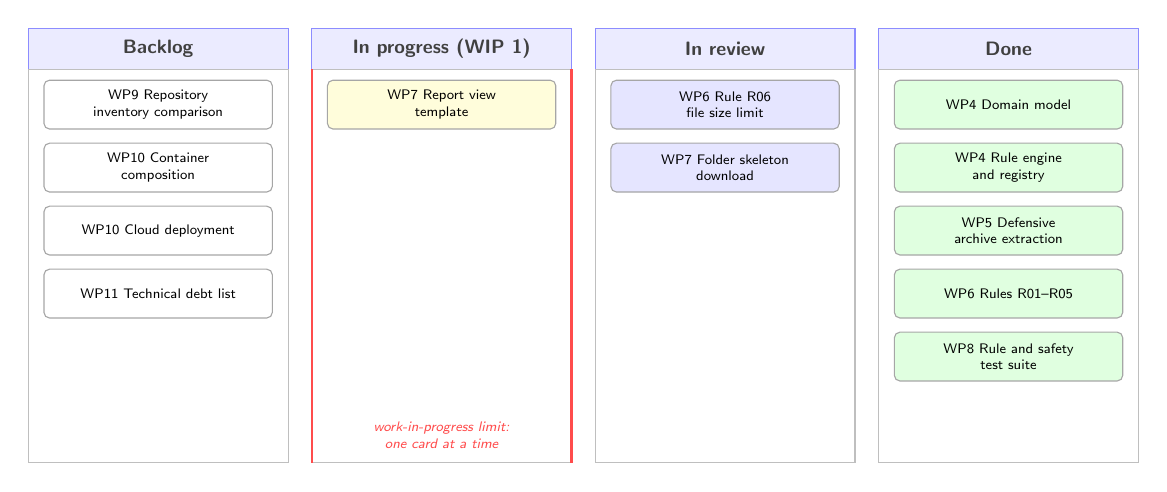
\begin{tikzpicture}[font=\scriptsize]
% Column headers and frames
\foreach \x/\title in {0/Backlog, 3.6/{In progress (WIP 1)}, 7.2/In review, 10.8/Done} {
  \fill[blue!8]  (\x,0.42) rectangle (\x+3.3,-0.1);
  \draw[blue!45] (\x,0.42) rectangle (\x+3.3,-0.1);
  \node[font=\scriptsize\bfseries, black!75] at (\x+1.65,0.16) {\title};
  \draw[black!25] (\x,-0.1) rectangle (\x+3.3,-5.1);
}
% Backlog
\node[card] at (1.65,-0.55) {WP9 Repository\\inventory comparison};
\node[card] at (1.65,-1.35) {WP10 Container\\composition};
\node[card] at (1.65,-2.15) {WP10 Cloud deployment};
\node[card] at (1.65,-2.95) {WP11 Technical debt list};
% In progress
\node[card, fill=yellow!14] at (5.25,-0.55) {WP7 Report view\\template};
% In review
\node[card, fill=blue!10] at (8.85,-0.55) {WP6 Rule R06\\file size limit};
\node[card, fill=blue!10] at (8.85,-1.35) {WP7 Folder skeleton\\download};
% Done
\node[card, fill=green!12] at (12.45,-0.55) {WP4 Domain model};
\node[card, fill=green!12] at (12.45,-1.35) {WP4 Rule engine\\and registry};
\node[card, fill=green!12] at (12.45,-2.15) {WP5 Defensive\\archive extraction};
\node[card, fill=green!12] at (12.45,-2.95) {WP6 Rules R01--R05};
\node[card, fill=green!12] at (12.45,-3.75) {WP8 Rule and safety\\test suite};
% WIP limit annotation
\draw[red!70, thick] (3.6,-0.1) -- (3.6,-5.1);
\draw[red!70, thick] (6.9,-0.1) -- (6.9,-5.1);
\node[font=\tiny\itshape, red!70, align=center] at (5.25,-4.75)
  {work-in-progress limit: \\ one card at a time};
\end{tikzpicture}
\caption{Kanban board at the end of the development phase}
\label{fig:kanban}
\end{figure}

\subsection{Supporting Engineering Practices}\label{subsec:practices}

Four practices support the methodology. Version control uses a public repository
with small, atomic commits and annotated tags marking the state submitted at
each portfolio milestone, so that release control is demonstrable from the
repository history itself \citep{Chacon2024}. Architecture documentation is
versioned alongside the source code so that the two cannot diverge silently
\citep{Bass2021}. Automated tests are written for every rule as part of the
increment that introduces it \citep{Khorikov2020}. Finally, any requirement that
cannot be met within the project scope is recorded explicitly as technical debt
rather than left unstated, because debt that is not written down cannot be
weighed against anything \citep{Winters2020}.

\section{Requirements}\label{sec:requirements}

\subsection{Specification Approach}\label{subsec:approach}

The requirements are derived directly from the assignment brief, which functions
as the authoritative specification of the domain: each formal provision
translates into one verifiable rule. This gives the project an unusual
advantage, since the requirements source is written and stable, but it also
imposes an obligation --- a rule that misreads its source produces confidently
wrong advice. Every rule therefore records the provision it derives from, and
that provenance is shown to the user so the rule can be checked against the
original document, maintaining the traceability from requirement to source that
requirements engineering demands \citep{Sommerville2020}.

Non-functional requirements are organised along the product quality
characteristics of ISO/IEC 25010, which supplies an established vocabulary and
keeps the list from collapsing into an unstructured set of aspirations
\citep{ISO25010}. The requirements base is presented in
Table~\ref{tab:requirements}. Its upper block lists the functional requirements
with a MoSCoW priority and the work package that delivers each; its lower block
lists the non-functional requirements, each labelled with its quality
characteristic and the means by which it is verified.

\begin{table}[H]
\centering
\caption{Functional and non-functional requirements, updated for the development phase}
\label{tab:requirements}
\footnotesize
\renewcommand{\arraystretch}{1.2}
\setlength{\tabcolsep}{4pt}
\begin{tabularx}{\textwidth}{|c|X|p{2.5cm}|c|}
\hline
\rowcolor{gray!15}
\textbf{ID} & \textbf{Requirement} & \textbf{Priority / Verification} & \textbf{WP} \\
\hline
\hline
\multicolumn{4}{|l|}{\cellcolor{blue!8}\textit{\textbf{Functional requirements}}} \\
\hline
FR1 & The system shall accept a submission archive uploaded through a web browser. & Must & WP5, WP7 \\
\hline
FR2 & The system shall verify the name of the main directory against the prescribed pattern. & Must & WP6 \\
\hline
FR3 & The system shall verify the presence and exact naming of all prescribed subdirectories. & Must & WP6 \\
\hline
FR4 & The system shall verify that files declared as PDF are genuinely PDF documents, by inspecting content rather than the file extension. & Must & WP6 \\
\hline
FR5 & The system shall verify that no file exceeds the prescribed size limit. & Must & WP6 \\
\hline
FR6 & The system shall verify the presence and content of the auxiliary artifacts required for the applicable phase. & Must & WP6 \\
\hline
FR7 & The system shall return a report giving each rule a verdict of \textit{passed}, \textit{to review} or \textit{must fix}. & Must & WP4 \\
\hline
FR8 & The system shall accompany every non-passing verdict with a concrete corrective action. & Must & WP4, WP7 \\
\hline
FR9 & The system shall allow the user to declare the portfolio phase and evaluate only the rules applicable to it. & Should & WP4 \\
\hline
FR10 & The system shall provide a downloadable, correctly structured but empty folder skeleton. & Should & WP7 \\
\hline
FR11 & The system shall display the provision of the brief from which each rule derives. & Should & WP7 \\
\hline
FR12 & The system shall compare the file inventory of the submitted code archive with that of the referenced public repository. & Could & WP9 \\
\hline
FR13 & The system shall expose the active rule catalogue, so that the set of rules being applied is inspectable before a submission is uploaded. & Should & WP6, WP7 \\
\hline
\hline
\multicolumn{4}{|l|}{\cellcolor{blue!8}\textit{\textbf{Non-functional requirements (ISO/IEC 25010 characteristics)}}} \\
\hline
NFR1 & \textit{Security.} The system shall reject archives containing absolute paths or relative path traversal before extraction. & Automated test, crafted archive & WP5 \\
\hline
NFR2 & \textit{Security.} The system shall reject archives whose expanded size, entry count or compression ratio exceeds defined limits. & Automated test, crafted archive & WP5 \\
\hline
NFR3 & \textit{Security.} The system shall delete every uploaded and extracted file before the response is returned, and persist no submission data. & Code review & WP5 \\
\hline
NFR4 & \textit{Security.} The application shall run without administrative privileges on a read-only container filesystem. & Configuration review & WP10 \\
\hline
NFR5 & \textit{Performance.} The system shall return a report within three seconds for a submission of typical size. & Timing during review & WP4 \\
\hline
NFR6 & \textit{Usability.} The report shall be comprehensible without reference to the assignment brief. & Review against FR8 & WP7 \\
\hline
NFR7 & \textit{Maintainability.} Adding a further rule shall require changes only to the rule component and its test. & Architecture review & WP4, WP6 \\
\hline
NFR8 & \textit{Reliability.} A failure in one rule shall not prevent the remaining rules from being evaluated. & Automated test & WP4 \\
\hline
NFR9 & \textit{Portability.} The system shall be deployable through a single container composition command. & Deployment from clean host & WP10 \\
\hline
\end{tabularx}
\end{table}

Requirement FR13 is new in this phase. It was added in response to the tutorial
question of how the rules reach the system, and is answered in
Section~\ref{subsec:ruleauthoring}. Requirement FR12 remains the principal source
of novelty: the brief requires the contents of the public repository and of the
submitted archive to be identical, a provision that is effectively impossible to
verify by hand and that no existing tool addresses \citep{Paiva2022}.

\subsection{Rule Definition and Maintenance}\label{subsec:ruleauthoring}

The tutorial feedback observed, correctly, that the conception document did not
say how a rule enters the system. The design decision is that
\textbf{rules are authored as code by the maintainer, not entered by end users},
and the reasoning deserves to be stated rather than assumed
\citep{Richards2020}.

A rule is not a data record. Verifying that a directory name matches a pattern,
that a declared PDF is genuinely a PDF, or that an archive inventory matches a
repository listing requires arbitrary logic, not a value in a form. Expressing
such logic through a configuration language would mean designing and
implementing a small rule language, together with its editor, its validation and
its error reporting --- an effort comparable to the whole of the rest of the
project, in exchange for a flexibility nobody in the target group has asked for
\citep{Sommerville2020}. Students are the users of the checker; they are not the
authors of the regulations it enforces, and giving them the power to edit the
rules would undermine the guarantee the tool exists to provide.

The rule lifecycle is therefore as follows. A provision of the assignment brief
is identified and recorded, together with the exact sentence it derives from. A
rule class is written implementing the common rule interface, declaring its
identifier, its title, the portfolio phases it applies to, and the provision it
references. A decorator registers the class with the rule registry at import
time, so no central list has to be edited and NFR7 is preserved. An automated
test is written that exercises the rule against a compliant submission and
against one violating exactly that rule. The rule then becomes visible in the
catalogue exposed by FR13, where a student can read the whole active rule set,
with its source provisions, before uploading anything. Defining the extension
point once, and requiring every extension to pass through it, is what keeps a
growing rule set from eroding the structure that holds it \citep{Percival2020}.

Three consequences follow, and each is a deliberate trade-off. Adding a rule
requires a redeployment rather than a configuration change, which is acceptable
because the regulations change at most once per academic period. The correctness
of a rule is guaranteed by its test rather than by user vigilance, which is the
stronger guarantee \citep{Khorikov2020}. And the cost of adding a rule is one
class plus one test, which is what makes the incremental plan in
Table~\ref{tab:workpackages} feasible. Should a future requirement call for
institution-specific rule sets, the registry is the single point at which that
change would be made.

\section{Glossary}\label{sec:glossary}

The glossary fixes the domain vocabulary so that a term carries the same meaning
for the developer, the tutor and any future reader; the entries are ordered
alphabetically, as the tutorial feedback requested \citep{Sommerville2020}.

\begin{description}[leftmargin=3.6cm, style=nextline, font=\normalfont\bfseries, itemsep=1pt]
\item[Corrective action] The concrete instruction accompanying a non-passing
finding, describing what must be changed for the rule to be satisfied.
\item[Finding] The verdict produced by evaluating one rule against one
submission: a severity, an explanatory message and, where applicable, a
corrective action.
\item[Main directory] The single top-level folder inside the submission
archive, whose name must follow the prescribed pattern.
\item[Phase] One of the three stages of the portfolio; determines which rules
apply to a given submission.
\item[Report] The aggregate of all findings for one submission, with the overall
verdict derived from the most severe finding.
\item[Rule] An independently verifiable formal requirement derived from one
provision of the assignment brief.
\item[Rule engine] The component that selects the applicable rules, evaluates
them against a submission and aggregates the resulting findings.
\item[Rule registry] The component that holds the active rule set and makes it
discoverable without any component having to know the individual rules.
\item[Severity] The classification of a finding as \textit{passed}, \textit{to
review} or \textit{must fix}.
\item[Submission] The complete set of files a student intends to hand in for one
portfolio phase, supplied to the system as a single archive.
\item[Technical debt] A requirement consciously left unsatisfied within the
project scope, recorded together with its consequence.
\end{description}

\section{Architecture Documentation}\label{sec:architecture}

\subsection{Scope and Context}\label{subsec:context}

The context view delimits the system from its environment. Presenting an
architecture as a small set of nested views --- the system in its environment
first, its internal structure second --- is a widely adopted convention, since
each view answers a different question and remains legible on its own
\citep{Brown2024}. Figure~\ref{fig:context} shows the boundary: the student is
the sole human user and interacts only through a web browser, the assignment
brief is the authoritative source from which the rule set is derived rather than
a runtime interface, and the repository hosting service is an optional interface
needed only by FR12 and therefore drawn with a dashed outline.

\begin{figure}[H]
\centering
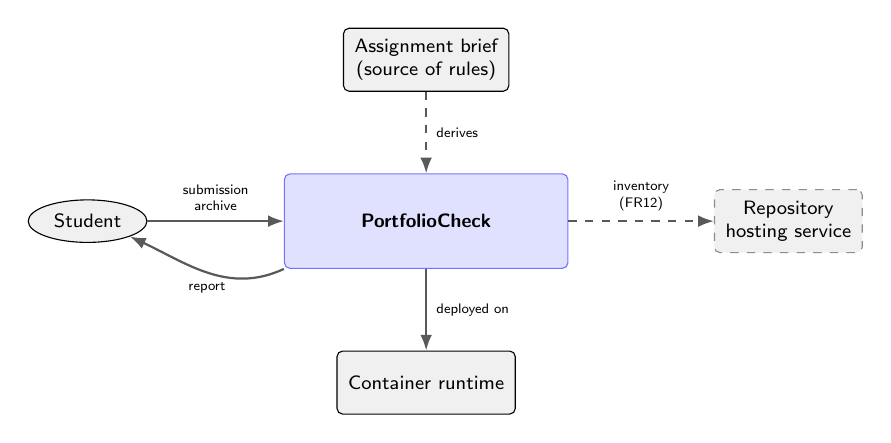
\begin{tikzpicture}
\node[system]                     at ( 0  , 0    ) (sys)  {PortfolioCheck};
\node[actor]                      at (-4.3, 0    ) (user) {Student};
\node[ext]                        at ( 0  , 2.05 ) (src)  {Assignment brief\\(source of rules)};
\node[ext, draw=black!45, dashed] at ( 4.6, 0    ) (opt)  {Repository\\hosting service};
\node[ext]                        at ( 0  ,-2.05 ) (host) {Container runtime};

\draw[flow] (user.east) -- node[above, font=\tiny, align=center] {submission\\archive} (sys.west);
\draw[flow] (sys.south west) to[out=205, in=335]
      node[below, font=\tiny] {report} (user.south east);
\draw[flow, dashed] (src.south) -- node[right, font=\tiny] {derives} (sys.north);
\draw[flow, dashed] (sys.east)  -- node[above, font=\tiny, align=center] {inventory\\(FR12)} (opt.west);
\draw[flow] (sys.south) -- node[right, font=\tiny] {deployed on} (host.north);
\end{tikzpicture}
\caption{System scope and context}
\label{fig:context}
\end{figure}

\subsection{Component View}\label{subsec:components}

The tutorial feedback asked for the internal structure to be expressed in a
standard notation. Figure~\ref{fig:components} is therefore a UML component
diagram: components carry the component icon, provided interfaces are shown as
lollipops, and dependencies on those interfaces are drawn as dashed arrows
\citep{Sommerville2020}. Naming the interfaces rather than merely the components
is what makes the diagram useful, since it is the interface, not the component,
that each dependency is actually bound to \citep{Richards2020}.

\begin{figure}[H]
\centering
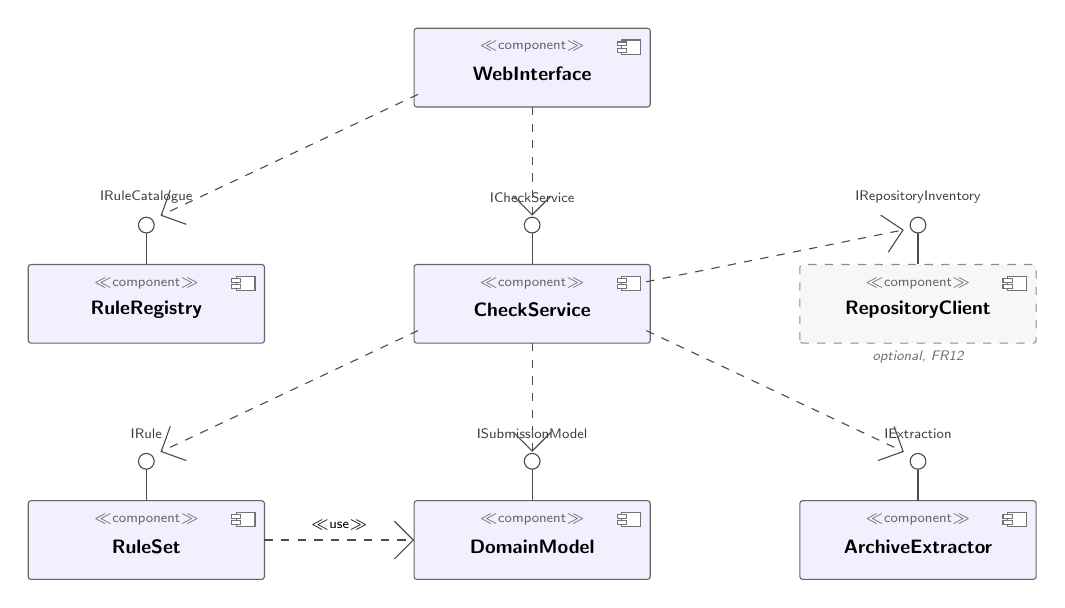
\begin{tikzpicture}[font=\scriptsize]
% ---- Components (w = 3.0, h = 1.0) ----
\foreach \cx/\cy/\name in {%
  6.5/0/WebInterface,
  1.6/-3/RuleRegistry,
  6.5/-3/CheckService,
  1.6/-6/RuleSet,
  6.5/-6/DomainModel,
  11.4/-6/ArchiveExtractor} {
  \draw[fill=blue!6, draw=black!60, rounded corners=1pt]
    (\cx-1.5,\cy-0.5) rectangle (\cx+1.5,\cy+0.5);
  \node[font=\tiny, black!60] at (\cx,\cy+0.26) {$\ll$component$\gg$};
  \node[font=\scriptsize\bfseries] at (\cx,\cy-0.08) {\name};
}
% Optional component, dashed border
\draw[fill=gray!6, draw=black!45, dashed, rounded corners=1pt]
  (9.9,-3.5) rectangle (12.9,-2.5);
\node[font=\tiny, black!60] at (11.4,-2.74) {$\ll$component$\gg$};
\node[font=\scriptsize\bfseries] at (11.4,-3.08) {RepositoryClient};
\node[font=\tiny\itshape, black!55] at (11.4,-3.68) {optional, FR12};

% ---- Component icons ----
\compicon{7.88}{0.26}
\compicon{2.98}{-2.74}
\compicon{7.88}{-2.74}
\compicon{12.78}{-2.74}
\compicon{2.98}{-5.74}
\compicon{7.88}{-5.74}
\compicon{12.78}{-5.74}

% ---- Provided interfaces (lollipops on top of the provider) ----
\foreach \lx/\ly/\lab in {%
  6.5/-2.5/ICheckService,
  1.6/-2.5/IRuleCatalogue,
  11.4/-2.5/IRepositoryInventory,
  1.6/-5.5/IRule,
  6.5/-5.5/ISubmissionModel,
  11.4/-5.5/IExtraction} {
  \draw[black!70] (\lx,\ly) -- (\lx,\ly+0.40);
  \draw[black!70, fill=white] (\lx,\ly+0.50) circle (0.10);
  \node[font=\tiny, anchor=south, black!75] at (\lx,\ly+0.66) {\lab};
}

% ---- Dependencies on interfaces ----
\draw[dep] (6.5,-0.5)  -- (6.5,-1.88);
\draw[dep] (5.05,-0.34) -- (1.78,-1.88);
\draw[dep] (5.05,-3.34) -- (1.78,-4.88);
\draw[dep] (6.5,-3.5)  -- (6.5,-4.88);
\draw[dep] (7.95,-3.34) -- (11.22,-4.88);
\draw[dep] (7.95,-2.72) -- (11.22,-2.06);
\draw[dep] (3.1,-6.0)  -- node[above, font=\tiny] {$\ll$use$\gg$} (5.0,-6.0);
\end{tikzpicture}
\caption{UML component diagram of the internal structure}
\label{fig:components}
\end{figure}

Six components and one optional component make up the system. \textbf{WebInterface}
accepts the upload, renders the report and publishes the rule catalogue; it
depends on \textit{ICheckService} and \textit{IRuleCatalogue} and on no
individual rule. \textbf{CheckService} is the rule engine: it obtains the
applicable rules through the registry, evaluates each against the submission and
aggregates the findings. \textbf{RuleRegistry} holds the active rule set and is
the single point at which a rule becomes known to the system.
\textbf{RuleSet} contains the individual rule classes. \textbf{DomainModel}
provides the Submission, Finding and Report types and depends on nothing.
\textbf{ArchiveExtractor} performs the defensive extraction, and
\textbf{RepositoryClient} realises the optional comparison of FR12. Each
component owns one responsibility and exposes it through a named interface,
which is the condition under which a component can later be replaced without its
consumers being rewritten \citep{Newman2021}.

The decomposition is driven directly by NFR7. Dependencies point inward toward
the domain model, which depends on nothing, so a rule can be added without any
other component changing \citep{Percival2020}. Keeping the domain model free of
any dependency on the web framework allows every rule to be tested against an
in-memory submission without starting a server, which is what makes the test
levels of Section~\ref{sec:testing} inexpensive enough to run on every change.
Extraction is confined to a single component because it is the one that touches
untrusted input, so the defences required by NFR1 and NFR2 are auditable in one
place rather than dispersed \citep{Newman2021}.

\subsection{Runtime View}\label{subsec:runtime}

The component diagram states which parts exist; it does not state the order in
which they act. Figure~\ref{fig:sequence} therefore adds a runtime view of the
central use case, a submission being checked, because a structural view alone
leaves the dynamics of a system undocumented \citep{Bass2021}.

\begin{figure}[H]
\centering
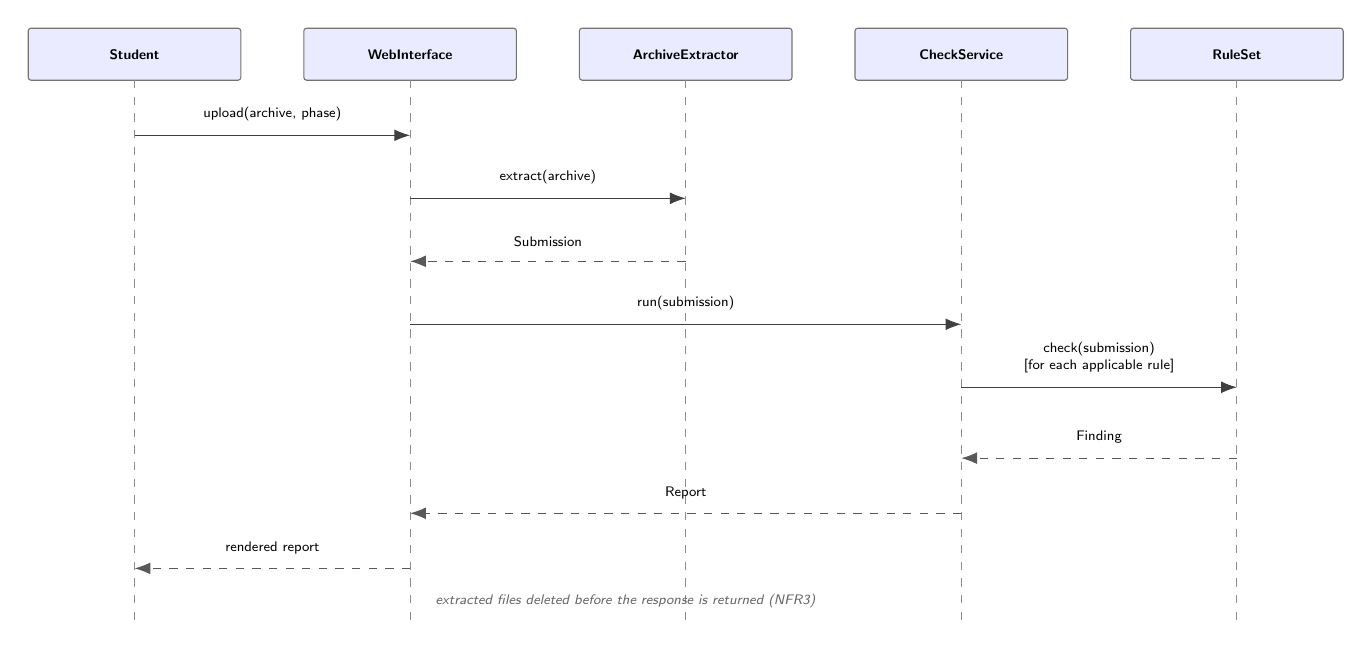
\begin{tikzpicture}[font=\scriptsize]
% Participants
\foreach \x/\name in {0/Student, 3.5/WebInterface, 7.0/ArchiveExtractor,
                      10.5/CheckService, 14.0/RuleSet} {
  \draw[fill=blue!8, draw=black!55, rounded corners=1pt]
    (\x-1.35,0) rectangle (\x+1.35,0.66);
  \node[font=\tiny\bfseries] at (\x,0.33) {\name};
  \draw[black!45, dashed] (\x,0) -- (\x,-6.9);
}
% Messages: from, to, y, label, style
\foreach \a/\b/\y/\lab in {%
  0/3.5/-0.7/{upload(archive, phase)},
  3.5/7.0/-1.5/{extract(archive)}} {
  \draw[-{Latex[length=2mm]}, black!75] (\a,\y) -- (\b,\y);
  \node[font=\tiny, anchor=south] at ({(\a+\b)/2},\y+0.06) {\lab};
}
\draw[-{Latex[length=2mm]}, dashed, black!65] (7.0,-2.3) -- (3.5,-2.3);
\node[font=\tiny, anchor=south] at (5.25,-2.24) {Submission};

\draw[-{Latex[length=2mm]}, black!75] (3.5,-3.1) -- (10.5,-3.1);
\node[font=\tiny, anchor=south] at (7.0,-3.04) {run(submission)};

\draw[-{Latex[length=2mm]}, black!75] (10.5,-3.9) -- (14.0,-3.9);
\node[font=\tiny, anchor=south, align=center] at (12.25,-3.84)
  {check(submission)\\{[for each applicable rule]}};

\draw[-{Latex[length=2mm]}, dashed, black!65] (14.0,-4.8) -- (10.5,-4.8);
\node[font=\tiny, anchor=south] at (12.25,-4.74) {Finding};

\draw[-{Latex[length=2mm]}, dashed, black!65] (10.5,-5.5) -- (3.5,-5.5);
\node[font=\tiny, anchor=south] at (7.0,-5.44) {Report};

\draw[-{Latex[length=2mm]}, dashed, black!65] (3.5,-6.2) -- (0,-6.2);
\node[font=\tiny, anchor=south] at (1.75,-6.14) {rendered report};

\node[font=\tiny\itshape, anchor=west, black!60] at (3.7,-6.62)
  {extracted files deleted before the response is returned (NFR3)};
\end{tikzpicture}
\caption{Runtime view: sequence of one submission check}
\label{fig:sequence}
\end{figure}

\subsection{Mapping Components to Source Code}\label{subsec:mapping}

The tutorial feedback asked that the components specified in the architecture be
findable in the source code as described. Table~\ref{tab:mapping} therefore maps
each component onto the module that realises it. Keeping this mapping explicit
is what prevents the documented architecture and the implemented one from
drifting apart, which is the ordinary fate of architecture documents that are
written once \citep{Bass2021}.

\begin{table}[H]
\centering
\caption{Mapping of architectural components to source modules}
\label{tab:mapping}
\footnotesize
\renewcommand{\arraystretch}{1.2}
\setlength{\tabcolsep}{4pt}
\begin{tabularx}{\textwidth}{|p{3.2cm}|p{4.2cm}|X|}
\hline
\rowcolor{gray!15}
\textbf{Component} & \textbf{Source module} & \textbf{Realised by} \\
\hline
\hline
WebInterface      & \texttt{app/main.py}, \texttt{app/templates/} & HTTP endpoints for upload, report, rule catalogue and folder skeleton \\
\hline
CheckService      & \texttt{app/checker.py}        & Selection of applicable rules, evaluation loop, aggregation into a Report \\
\hline
RuleRegistry      & \texttt{app/rules/base.py}     & Rule base class and the registration decorator that populates the catalogue \\
\hline
RuleSet           & \texttt{app/rules/naming.py}, \texttt{structure.py}, \texttt{artifacts.py}, \texttt{integrity.py} & One module per group of related rules; one class per rule \\
\hline
DomainModel       & \texttt{app/models.py}         & Submission, SubmissionFile, Finding, Severity and Report types \\
\hline
ArchiveExtractor  & \texttt{app/extraction.py}     & Archive inspection against the safety limits and extraction to a temporary directory \\
\hline
RepositoryClient  & planned, WP9                   & Inventory retrieval from the repository hosting service (FR12) \\
\hline
\end{tabularx}
\end{table}

\section{Technology Stack and Third-Party Libraries}\label{sec:stack}

\subsection{Decisions and the Alternatives Considered}\label{subsec:alternatives}

The tutorial feedback asked for the technology stack to be explained in more
detail, and in particular for the alternatives with similar characteristics to
be addressed. Table~\ref{tab:alternatives} therefore records, for each decision,
what was selected, what was considered instead, and the reason the alternative
was set aside. Recording the discarded options alongside the chosen one is what
makes an architectural decision reviewable later, since a decision without its
rejected alternatives cannot be re-evaluated when the context changes
\citep{Ford2021}.

\begin{table}[H]
\centering
\caption{Technology decisions, alternatives considered and rationale}
\label{tab:alternatives}
\footnotesize
\renewcommand{\arraystretch}{1.2}
\setlength{\tabcolsep}{4pt}
\begin{tabularx}{\textwidth}{|p{2.3cm}|p{2.2cm}|p{2.9cm}|X|}
\hline
\rowcolor{gray!15}
\textbf{Decision} & \textbf{Selected} & \textbf{Alternatives considered} & \textbf{Rationale for the choice} \\
\hline
\hline
Language & Python 3.11 & Java, Node.js & The problem domain is archive and document inspection, which the Python standard library covers directly with \texttt{zipfile} \citep{PSF2025}. Java offers comparable libraries but a heavier build chain for a single developer; Node.js would have required a third-party archive library for what is here a built-in. \\
\hline
Web framework & FastAPI \citep{FastAPI2025} & Flask \citep{Flask2025}, Django \citep{Django2025} & All three could serve this application. Django brings an ORM, an admin interface and a migration system, none of which are used since the system has no database (NFR3); adopting it would mean carrying a large framework for its routing alone. Flask is comparably light, but FastAPI adds declarative request and upload validation at the boundary, which is exactly where untrusted input arrives (NFR1, NFR2). \\
\hline
User interface & Server-rendered Jinja templates \citep{Jinja2025} & Single-page application in React or Vue & The interface is one form and one report. A client-side application would add a build pipeline, a second deployment artifact and a client-server contract to maintain, in exchange for interactivity the use case does not require \citep{Richards2020}. \\
\hline
ASGI server & Uvicorn \citep{Uvicorn2025} & Gunicorn with worker classes, Hypercorn & Uvicorn is the reference server for the chosen framework and is configured in a single command line; the alternatives add process-management features that matter at a scale this application does not reach. \\
\hline
Persistence & None & SQLite, PostgreSQL & No requirement calls for retaining submissions, and NFR3 forbids it. Omitting persistence removes a component, a schema, a backup concern and a data-protection obligation. Should a history feature ever be required, the layered decomposition confines the change to the infrastructure layer. \\
\hline
Testing & pytest \citep{Pytest2025} & \texttt{unittest} from the standard library & Both execute the same tests. pytest was chosen for parameterised test cases, which suit a rule set where each rule is exercised against a compliant and a violating submission, and for fixtures that build a submission from a plain mapping of paths to content \citep{Khorikov2020}. \\
\hline
Packaging & Docker Compose \citep{Docker2024} & Bare virtual environment on the host & Required by the brief, and it guarantees that the environment described in the documentation is the environment that runs (NFR9). It also carries the hardening required by NFR4 as declarative configuration rather than as deployment instructions. \\
\hline
\end{tabularx}
\end{table}

\subsection{Third-Party Libraries}\label{subsec:libraries}

Table~\ref{tab:libraries} lists every third-party library the application
depends on, with its purpose, its licence and a hyperlink to its documentation.
Recording licences alongside dependencies is part of maintaining a project that
others could take over, rather than an administrative afterthought
\citep{Winters2020}.

\begin{table}[H]
\centering
\caption{Third-party libraries, purpose, licence and references}
\label{tab:libraries}
\footnotesize
\renewcommand{\arraystretch}{1.2}
\setlength{\tabcolsep}{4pt}
\begin{tabularx}{\textwidth}{|p{2.3cm}|X|p{1.9cm}|p{3.4cm}|}
\hline
\rowcolor{gray!15}
\textbf{Library} & \textbf{Purpose in this project} & \textbf{Licence} & \textbf{Reference} \\
\hline
\hline
FastAPI & HTTP routing, multipart upload handling and request validation at the system boundary & MIT & \url{https://fastapi.tiangolo.com/} \\
\hline
Uvicorn & ASGI server that runs the application inside the container & BSD-3-Clause & \url{https://www.uvicorn.org/} \\
\hline
Jinja & Server-side rendering of the upload form, the report and the rule catalogue & BSD-3-Clause & \url{https://jinja.palletsprojects.com/} \\
\hline
python-multipart & Parsing of the multipart request carrying the uploaded archive & Apache-2.0 & \url{https://github.com/Kludex/python-multipart} \\
\hline
pytest & Execution of the rule, extraction and interface test suites & MIT & \url{https://docs.pytest.org/} \\
\hline
httpx & Transport used by the test client to exercise the HTTP interface & BSD-3-Clause & \url{https://www.python-httpx.org/} \\
\hline
\end{tabularx}
\end{table}

No third-party library is used for archive handling itself. The Python standard
library provides \texttt{zipfile}, and the defensive limits required by NFR1 and
NFR2 are implemented directly on top of it, so that the component which touches
untrusted input contains no code the project does not control
\citep{PSF2025}.

\section{Design and Implementation Procedure}\label{sec:procedure}

Implementation proceeded outward from the centre of the component diagram. The
domain model was built first, because every other component depends on it and
nothing depends on it in turn; expressing Submission, Finding, Severity and
Report as small immutable types meant that the rest of the system could be
written against a stable vocabulary \citep{Percival2020}. One design decision
was taken at this point and deserves recording: a finding whose severity is
worse than \textit{passed} is required by construction to carry a corrective
action, and the type raises if one is constructed without it. FR8 is thereby
enforced by the model rather than left to the discipline of whoever writes the
next rule \citep{Khorikov2020}.

The rule abstraction and the registry followed. A rule declares its identifier,
its title, the phases it applies to and the provision of the brief it derives
from, and implements a single evaluation method returning one or more findings.
Registration happens through a decorator, so that adding a rule touches only the
new module and no central list, which is the concrete form NFR7 takes in the
code \citep{Richards2020}.

Archive extraction was implemented next, ahead of any rule, because it is the
component that receives untrusted input and because the remaining work depends
on having a safely extracted submission to operate on. The archive is inspected
before anything is written to disk: entries with absolute paths or traversal
segments are rejected, as are archives exceeding the entry-count, expanded-size
and per-entry compression-ratio limits \citep{OWASP2021}. This ordering was
deliberate. Implementing the rules first and the defences afterwards would have
meant running untrusted archives through an unhardened path during development,
which is how such defences come to be retrofitted rather than designed
\citep{NIST2022}.

The rule set was then grown one rule at a time, each with its test, in the order
given by WP6. Two rules are worth noting for their design. The integrity rule
inspects the leading bytes of a file rather than its extension, since a document
renamed to end in \texttt{.pdf} is precisely the failure the examiner would
encounter and the extension is therefore not evidence. The structure rule, when
a prescribed directory is absent, searches for a folder differing only in case
or separators and names it in the finding, because the common failure is a
near-miss rather than an omission and the corrective action is far more useful
when it identifies the folder actually present \citep{Combefis2022}.

The web interface was implemented last, deliberately, so that it could be written
against a rule engine that already worked. It discovers the rule set through the
registry rather than naming rules individually, which is what allows the rule
catalogue of FR13 to stay correct as rules are added \citep{Richards2020}.
Uploads are streamed to a temporary directory with a size ceiling applied during
the write rather than after it, and the directory is removed in a \texttt{finally}
block so that NFR3 holds on the error path as well as the success path.

\section{Test Strategy}\label{sec:testing}

Verification was planned during conception and elaborated in this phase, in
keeping with the principle that requirements and their means of verification
belong together \citep{Khorikov2020}. Table~\ref{tab:testing} states the test
levels, what each establishes and the requirements it covers.

\begin{table}[H]
\centering
\caption{Test levels, objectives and requirement coverage}
\label{tab:testing}
\footnotesize
\renewcommand{\arraystretch}{1.2}
\setlength{\tabcolsep}{4pt}
\begin{tabularx}{\textwidth}{|p{2.9cm}|X|p{2.6cm}|}
\hline
\rowcolor{gray!15}
\textbf{Test level} & \textbf{Objective} & \textbf{Requirements} \\
\hline
\hline
Rule unit tests & Each rule is exercised against a compliant submission and against a submission violating exactly that rule, so that a rule cannot pass by failing to fire. & FR2--FR6, FR9, FR13 \\
\hline
Extraction safety tests & Crafted archives containing traversal segments, absolute paths, excessive entry counts and extreme compression ratios confirm that each limit is enforced before extraction. & NFR1, NFR2 \\
\hline
Interface tests & The complete upload-to-report path is exercised through the HTTP interface, including rejection of non-archive and corrupt uploads. & FR1, FR7, FR8, FR10 \\
\hline
Resilience test & A deliberately failing rule confirms that the remaining rules are still evaluated and that the report is still produced. & NFR8 \\
\hline
Deployment test & The application is started from a clean environment through the container composition and answers a health request. & NFR9 \\
\hline
\end{tabularx}
\end{table}

Test data consists of submission archives modelled on genuine portfolio
structures rather than placeholder content, built from a plain mapping of paths
to file content so that each test reads as a description of the folder it
exercises. A test is only as convincing as the representativeness of the data it
runs against, and a checker validated solely against synthetic input would
demonstrate very little about real submissions \citep{Khorikov2020}.

\section{Technical Debt and Outlook}\label{sec:debt}

Three items of technical debt are recorded at the close of this phase, each with
the consequence of leaving it unpaid, since debt that is acknowledged can be
weighed while debt that is silent cannot \citep{Winters2020}. First, the rule
set covers the provisions of one institution's brief and the identifiers are
embedded in the rule classes; supporting a second institution would require the
registry to become rule-set-aware. Second, the size and structural limits applied
during extraction are compiled-in constants rather than configuration, so
adjusting them requires a redeployment. Third, the repository comparison of FR12
is specified and scheduled but not yet implemented, so the provision requiring
the archive and the repository to be identical remains unverified by the tool.

The finalisation phase will complete WP9 through WP11: the repository inventory
comparison, the container composition and cloud deployment required by NFR4 and
NFR9, and the installation and run instructions. The architecture documentation
will be updated should those work packages change the decomposition, and the
mapping in Table~\ref{tab:mapping} will be extended as the RepositoryClient
component moves from planned to realised, so that the documented architecture
continues to describe the system that actually exists \citep{Ford2021}.

\newpage

% =====================================================================
% REFERENCES
% =====================================================================
\section*{References}
\addcontentsline{toc}{section}{References}

\begin{thebibliography}{99}
\setlength{\itemsep}{5pt}

\bibitem[Ambler and Lines(2022)]{Ambler2022}
Ambler, S. W. and Lines, M. (2022) \textit{Choose Your WoW! A Disciplined Agile
Approach to Optimizing Your Way of Working}. 2nd edn. Newtown Square, PA:
Project Management Institute.

\bibitem[Bass et~al.(2021)]{Bass2021}
Bass, L., Clements, P. and Kazman, R. (2021) \textit{Software Architecture in
Practice}. 4th edn. Boston, MA: Addison-Wesley.

\bibitem[Brown(2024)]{Brown2024}
Brown, S. (2024) \textit{The C4 Model for Visualising Software Architecture}.
Available at: \url{https://c4model.com/} (Accessed: 12 September 2026).

\bibitem[Chacon and Straub(2024)]{Chacon2024}
Chacon, S. and Straub, B. (2024) \textit{Pro Git}. 2nd edn (continuously
updated). Available at: \url{https://git-scm.com/book/} (Accessed:
12 September 2026).

\bibitem[Comb\'{e}fis(2022)]{Combefis2022}
Comb\'{e}fis, S. (2022) `Automated code assessment for education: review,
classification and perspectives on techniques and tools', \textit{Software},
1(1), pp. 3--30.

\bibitem[Django Software Foundation(2025)]{Django2025}
Django Software Foundation (2025) \textit{Django Documentation}. Available at:
\url{https://docs.djangoproject.com/} (Accessed: 12 September 2026).

\bibitem[Docker(2024)]{Docker2024}
Docker Inc. (2024) \textit{Compose Specification}. Available at:
\url{https://docs.docker.com/compose/} (Accessed: 12 September 2026).

\bibitem[Encode(2025)]{Uvicorn2025}
Encode (2025) \textit{Uvicorn: An ASGI Web Server for Python}. Available at:
\url{https://www.uvicorn.org/} (Accessed: 12 September 2026).

\bibitem[Ford et~al.(2021)]{Ford2021}
Ford, N., Richards, M., Sadalage, P. and Dehghani, Z. (2021) \textit{Software
Architecture: The Hard Parts --- Modern Trade-Off Analyses for Distributed
Architectures}. Sebastopol, CA: O'Reilly Media.

\bibitem[Hermans(2021)]{Hermans2021}
Hermans, F. (2021) \textit{The Programmer's Brain: What Every Programmer Needs
to Know about Cognition}. Shelter Island, NY: Manning.

\bibitem[ISO/IEC(2023)]{ISO25010}
International Organization for Standardization (2023) \textit{ISO/IEC
25010:2023 Systems and Software Engineering --- Systems and Software Quality
Requirements and Evaluation (SQuaRE) --- Product Quality Model}. Geneva: ISO.

\bibitem[Khorikov(2020)]{Khorikov2020}
Khorikov, V. (2020) \textit{Unit Testing Principles, Practices, and Patterns}.
Shelter Island, NY: Manning.

\bibitem[Messer et~al.(2024)]{Messer2024}
Messer, M., Brown, N. C. C., K\"{o}lling, M. and Shi, M. (2024) `Automated
grading and feedback tools for programming education: a systematic review',
\textit{ACM Transactions on Computing Education}, 24(1), pp. 1--43.

\bibitem[Newman(2021)]{Newman2021}
Newman, S. (2021) \textit{Building Microservices: Designing Fine-Grained
Systems}. 2nd edn. Sebastopol, CA: O'Reilly Media.

\bibitem[NIST(2022)]{NIST2022}
National Institute of Standards and Technology (2022) \textit{SP 800-218:
Secure Software Development Framework (SSDF) Version 1.1}. Gaithersburg, MD:
NIST.

\bibitem[OWASP(2021)]{OWASP2021}
Open Worldwide Application Security Project (2021) \textit{OWASP Top 10:2021}.
Available at: \url{https://owasp.org/Top10/} (Accessed: 12 September 2026).

\bibitem[Paiva et~al.(2022)]{Paiva2022}
Paiva, J. C., Leal, J. P. and Figueira, \'{A}. (2022) `Automated assessment in
computer science education: a state-of-the-art review', \textit{ACM
Transactions on Computing Education}, 22(3), pp. 1--40.

\bibitem[Pallets(2025a)]{Flask2025}
Pallets Projects (2025) \textit{Flask Documentation}. Available at:
\url{https://flask.palletsprojects.com/} (Accessed: 12 September 2026).

\bibitem[Pallets(2025b)]{Jinja2025}
Pallets Projects (2025) \textit{Jinja Documentation}. Available at:
\url{https://jinja.palletsprojects.com/} (Accessed: 12 September 2026).

\bibitem[Percival and Gregory(2020)]{Percival2020}
Percival, H. and Gregory, B. (2020) \textit{Architecture Patterns with Python}.
Sebastopol, CA: O'Reilly Media.

\bibitem[pytest-dev(2025)]{Pytest2025}
pytest-dev Team (2025) \textit{pytest Documentation}. Available at:
\url{https://docs.pytest.org/} (Accessed: 12 September 2026).

\bibitem[Python Software Foundation(2025)]{PSF2025}
Python Software Foundation (2025) \textit{zipfile --- Work with ZIP Archives.
Python 3.11 Standard Library Documentation}. Available at:
\url{https://docs.python.org/3/library/zipfile.html} (Accessed:
12 September 2026).

\bibitem[Ram\'{i}rez(2025)]{FastAPI2025}
Ram\'{i}rez, S. (2025) \textit{FastAPI Documentation}. Available at:
\url{https://fastapi.tiangolo.com/} (Accessed: 12 September 2026).

\bibitem[Richards and Ford(2020)]{Richards2020}
Richards, M. and Ford, N. (2020) \textit{Fundamentals of Software Architecture:
An Engineering Approach}. Sebastopol, CA: O'Reilly Media.

\bibitem[Schwaber and Sutherland(2020)]{Schwaber2020}
Schwaber, K. and Sutherland, J. (2020) \textit{The Scrum Guide: The Definitive
Guide to Scrum}. Available at: \url{https://scrumguides.org/} (Accessed:
12 September 2026).

\bibitem[Sommerville(2020)]{Sommerville2020}
Sommerville, I. (2020) \textit{Engineering Software Products: An Introduction
to Modern Software Engineering}. Harlow: Pearson Education.

\bibitem[Winters et~al.(2020)]{Winters2020}
Winters, T., Manshreck, T. and Wright, H. (2020) \textit{Software Engineering
at Google: Lessons Learned from Programming over Time}. Sebastopol, CA:
O'Reilly Media.

\end{thebibliography}

\end{document}
